% PyQCU — 鲲鹏真实环境进展图表（2026-11-10）
% 源数据：docs/kupl_kunpeng_progress_20261110.md 与其引用的日志。
% 编译（两遍）：
%   xelatex -interaction=nonstopmode -halt-on-error kupl_kunpeng_figures_20261110.tex
% 验收门：Overfull=0、Float too large=0、Missing character=0（已实测通过）。
%
% 两条作图规则（本文件强制）：
%   1) 所有对数轴的柱标签一律用 point meta=explicit + meta 列输出真实数值，
%      否则 pgfplots 默认打印 log10 值（例如 0.435 会被打成 -0.4）。
%   2) 误差条只表示样本内 min–max 的半幅，不是置信区间；每图必须写明 n 与口径。
\documentclass[10pt]{article}
\usepackage[a4paper,margin=16mm]{geometry}
\usepackage{ctex}
\usepackage{pgfplots}
\usepackage{booktabs}
\usepackage{tabularx}
\usepackage{array}
\usepackage{float}
\usepackage[hidelinks]{hyperref}
\pgfplotsset{compat=1.18}
% 本机未安装 TeX Gyre / Fandol，使用 ctex 的 macOS 字体集；
% 跨机复现时若需指定字体，先确认字体存在再启用 \setmainfont/\setCJKmainfont。
\newlength{\figw}\setlength{\figw}{0.96\linewidth}
\pgfplotsset{
  every axis/.append style={font=\scriptsize},
  every axis label/.append style={font=\small},
  nodes near coords/.append style={font=\tiny,inner sep=1pt},
}
\pagestyle{plain}
\title{KUPL 鲲鹏真实环境进展：数据图表\\\large 2026-11-05 至 2026-11-10（未打 tag，时点证据）}
\author{PyQCU}
\date{2026-11-10}

\begin{document}
\maketitle

\noindent\textbf{读图约定}
\begin{itemize}\itemsep1pt
  \item 耗时单位秒（s）；带宽 GB/s（十进制）；利用率百分数。
  \item 柱上标注样本数或真实数值；$n{=}1$ 一律视为单样本，不代表中位数。
  \item 范围值 $a$--$b$ 画为 $(a+b)/2$ 加 $\pm(b-a)/2$ 的误差条，只表示样本内最小--最大，\emph{不是}置信区间。
  \item 计算节点 \texttt{cn10579}（SVE2，16 CPU NUMA + 16 片上 NUMA，cpuset 上界 577）与登录节点 \texttt{login02/03}（Kunpeng-920，无 SVE，4 NUMA，共享机，无片上内存域）硬件不同，禁止跨类比较绝对值。
  \item 图注给出配置、窗口与证据边界；缺失项写“未验证”，不用估计值补位。
  \item 数据等级见第 7 节台账：\textbf{A}＝本地可复现原文；\textbf{B}＝阶段日志转述；\textbf{C}＝文档转述。
\end{itemize}

\tableofcontents
\vspace{4mm}

\section{绝对耗时与相对基线加速比}

\begin{figure}[H]
\centering
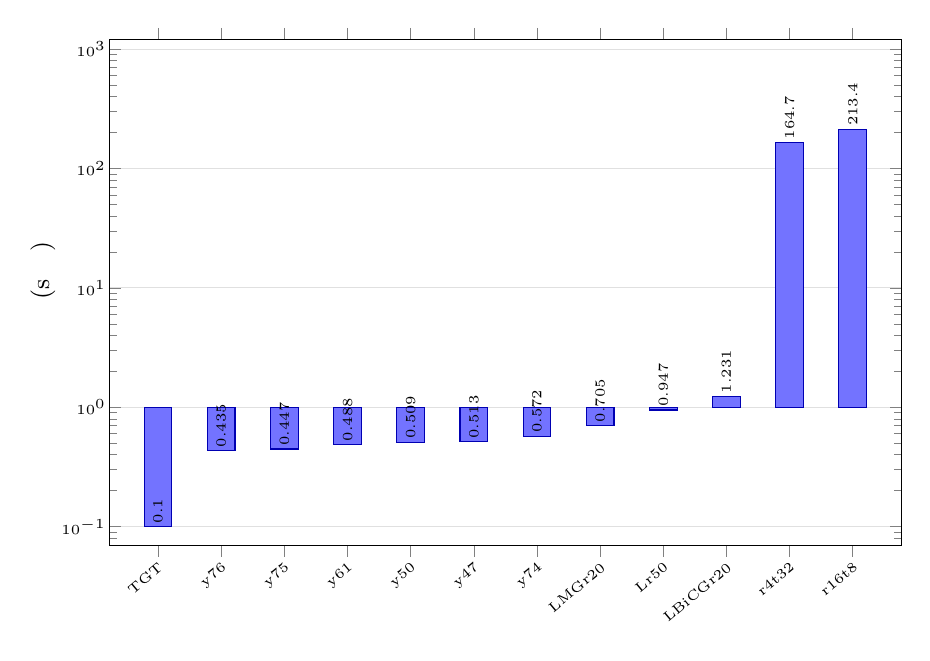
\begin{tikzpicture}
\begin{axis}[
  width=\figw, height=8.0cm,
  ybar, bar width=10pt, ymode=log, log basis y=10,
  ymin=0.07, ymax=1200,
  ylabel={求解段墙钟 (s，对数轴)},
  xlabel={配置},
  symbolic x coords={TGT,y76,y75,y61,y50,y47,y74,LMGr20,Lr50,LBiCGr20,r4t32,r16t8},
  xtick=data,
  xticklabel style={rotate=40,anchor=north east},
  ymajorgrids, grid style={black!12},
  point meta=explicit symbolic,
  nodes near coords, nodes near coords style={rotate=90,anchor=west},
  enlarge x limits=0.07,
]
\addplot[fill=blue!55,draw=blue!70!black] table[meta=lab] {
  x        y            lab
  TGT      0.1          0.1
  y76      0.43456275   0.435
  y75      0.4472       0.447
  y61      0.4877       0.488
  y50      0.5093       0.509
  y47      0.5126       0.513
  y74      0.5719       0.572
  LMGr20   0.705146     0.705
  Lr50     0.947332     0.947
  LBiCGr20 1.230783     1.231
  r4t32    164.7499     164.7
  r16t8    213.4409     213.4
};
\end{axis}
\end{tikzpicture}
\caption{绝对耗时（对数轴；柱上为真实秒数，不是 log10）。\textbf{计算节点} \texttt{cn10579}：y76 $=0.43456$ s（32 ranks$\times$12 threads，\texttt{grid} $1\,1\,1\,32$，16 迭代，独立真残差 $3.5412\times10^{-6}$，$n{=}1$）；y75 $=0.44720$ s（同配置，\texttt{atol}$=10^{-4}$，16 迭代，$n{=}1$）；y61 $=0.48770$ s（剖析同轮）；y50 $=0.5093$ s；y47 $=0.5126$ s；y74 $=0.57190$ s（\texttt{atol}$=10^{-5}$，18 迭代，$n{=}1$）；4 ranks$\times$32 threads $=164.74992$ s（作业 2049318，16 迭代，\emph{仅} native 残差 $1.237\times10^{-5}$，\emph{未}做独立残差）；16 ranks$\times$8 threads $=213.44091$ s（作业 2050917，\texttt{grid} $1\,1\,1\,16$，16 迭代，独立真残差 $3.5411\times10^{-6}$ PASS）。\textbf{登录节点}（共享机）：LBiCGr20 $=1.23078$ s、LMGr20 $=0.70515$ s（同窗 $n{=}4$ 中位，\texttt{cc}=9、\texttt{fc}=29）；Lr50 $=0.94733$ s（full-residual 伴随运行，只执行 1 次 coarse correction）。\textbf{口径警告}：16r$\times$8t / 4r$\times$32t 与 y76 的 ranks/threads/每 rank 局部体积不同，$213.44/0.43456=491\times$ 不能归因于 HBM 是否生效；只有 y76/y75/y61/y50/y47/y74 属同一 32$\times$12 几何。}
\end{figure}

\begin{figure}[H]
\centering
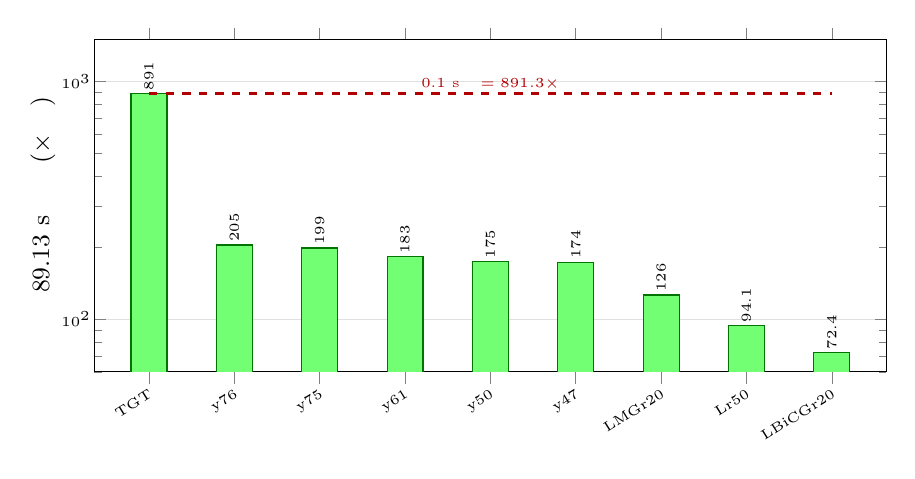
\begin{tikzpicture}
\begin{axis}[
  width=\figw, height=5.8cm,
  ybar, bar width=13pt, ymode=log, log basis y=10,
  ymin=60, ymax=1500,
  ylabel={相对 89.13 s 基线加速比 ($\times$，对数轴)},
  xlabel={配置},
  symbolic x coords={TGT,y76,y75,y61,y50,y47,LMGr20,Lr50,LBiCGr20},
  xtick=data,
  xticklabel style={rotate=32,anchor=north east},
  ymajorgrids, grid style={black!12},
  point meta=explicit symbolic,
  nodes near coords, nodes near coords style={rotate=90,anchor=west},
  enlarge x limits=0.08,
]
\addplot[fill=green!55,draw=green!45!black] table[meta=lab] {
  x        y       lab
  TGT      891.30  891
  y76      205.10  205
  y75      199.32  199
  y61      182.76  183
  y50      175.00  175
  y47      173.88  174
  LMGr20   126.40  126
  Lr50     94.09   94.1
  LBiCGr20 72.42   72.4
};
\draw[dashed,red!70!black,thick] (axis cs:TGT,891.30) -- (axis cs:LBiCGr20,891.30)
  node[midway,above,font=\tiny,text=red!70!black]{0.1 s 目标 $=891.3\times$};
\end{axis}
\end{tikzpicture}
\caption{相对 \textbf{89.13 s} 原始基线的加速比。原始基线为 4 ranks$\times$32 threads、无 NUMA 映射、HBM 未生效、OpenMP 线程挤单核的历史运行；\emph{本地不存在原始 report.json}，来源为日志转述（\texttt{logs/kupl\_qcu\_mg\_instructions\_20261105.txt}、\texttt{logs/resume-20261105T080514.gnF1tz.txt}），等级 C。该倍率混合了四项修复的合计效果（\texttt{set\_mempolicy} 掩码对齐、逐线程绑核、NUMA 映射、rank-local slab），不是单项优化收益。登录节点两柱由登录节点中位折算，只表示量级，不与计算节点作性能比较。}
\end{figure}

\section{计算节点作业台账与几何不可比性}

\begin{figure}[H]
\centering
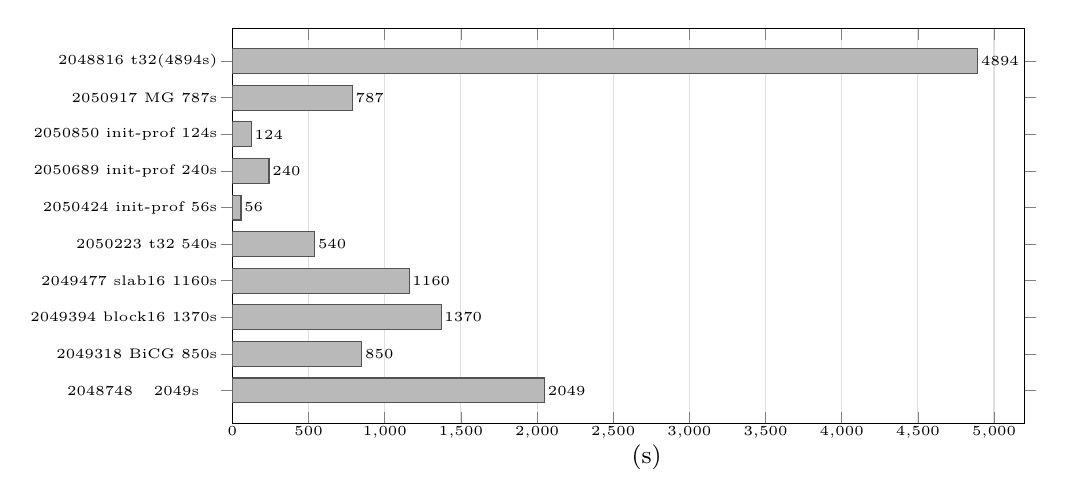
\begin{tikzpicture}
\begin{axis}[
  width=\figw, height=6.6cm,
  xbar, bar width=9pt,
  xmin=0, xmax=5200,
  xlabel={作业墙钟 (s)},
  symbolic y coords={J2048748,J2049318,J2049394,J2049477,J2050223,J2050424,J2050689,J2050850,J2050917,J2048816},
  ytick=data,
  yticklabels={%
    2048748 探针 2049s 无输出,%
    2049318 BiCG 850s,%
    2049394 block16 1370s,%
    2049477 slab16 1160s,%
    2050223 t32 540s,%
    2050424 init-prof 56s,%
    2050689 init-prof 240s,%
    2050850 init-prof 124s,%
    2050917 MG 787s,%
    2048816 t32(4894s)},
  yticklabel style={align=right},
  xmajorgrids, grid style={black!12},
  point meta=explicit symbolic,
  nodes near coords, nodes near coords style={anchor=west},
  enlarge y limits=0.10,
]
\addplot[fill=gray!55,draw=gray!65!black] table[meta=lab] {
  x     y          lab
  2049  J2048748   2049
  850   J2049318   850
  1370  J2049394   1370
  1160  J2049477   1160
  540   J2050223   540
  56    J2050424   56
  240   J2050689   240 (rc=124)
  124   J2050850   124 (rc=0)
  787   J2050917   787 (exit 143)
  4894  J2048816   4894 (exit 143)
};
\end{axis}
\end{tikzpicture}
\caption{计算节点作业墙钟台账（全部为本地可复现的调度器记录，等级 A）。\textbf{唯一完成求解的作业是两个}：2049318（4$\times$32，BiCGStab 164.75 s，native 残差 $1.237\times10^{-5}$，独立残差跳过）与 2050917（16$\times$8，BiCGStab 213.44 s，独立真残差 $3.5411\times10^{-6}$ PASS）；后者的配对 MG case 在 787 s 无 \texttt{report.json}，经同队列本账号 TERM kill-job（2051058）终止，\texttt{jobExitCode=143}。2050850 是唯一 \texttt{END rc=0} 的完整初始化剖析作业（124 s）；2050689 在 240 s 内部超时（\texttt{rc=124}）。2048748 探针被接受并调度到 \texttt{cn10579}，但声明的 \texttt{y79.out} 路径未生成。\textbf{审计规则}：满 5 分钟查日志与进度，满 10 分钟且不能证明健康即终止并全面审查；未绕过 hook、未绕过 host-key、未操作其他用户进程。}
\end{figure}

\begin{figure}[H]
\centering
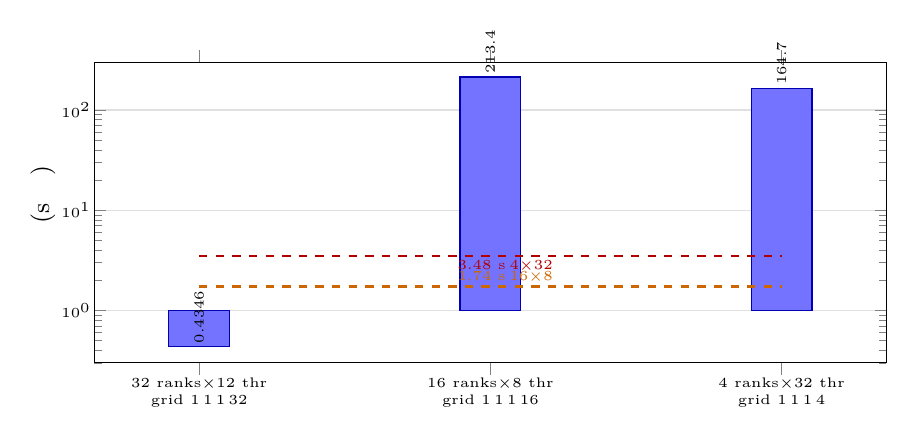
\begin{tikzpicture}
\begin{axis}[
  width=\figw, height=5.4cm,
  ybar, bar width=22pt, ymode=log, log basis y=10,
  ymin=0.3, ymax=300,
  ylabel={求解墙钟 (s，对数轴)},
  symbolic x coords={p32x12,p16x8,p4x32},
  xtick=data,
  xticklabels={{32 ranks$\times$12 thr\\grid $1\,1\,1\,32$},{16 ranks$\times$8 thr\\grid $1\,1\,1\,16$},{4 ranks$\times$32 thr\\grid $1\,1\,1\,4$}},
  xticklabel style={align=center},
  ymajorgrids, grid style={black!12},
  point meta=explicit symbolic,
  nodes near coords, nodes near coords style={rotate=90,anchor=west},
  enlarge x limits=0.18,
]
\addplot[fill=blue!55,draw=blue!70!black] table[meta=lab] {
  x      y          lab
  p32x12 0.43456275 0.4346
  p16x8  213.4409   213.4
  p4x32  164.7499   164.7
};
\draw[dashed,orange!80!black,thick] (axis cs:p32x12,1.73825) -- (axis cs:p4x32,1.73825)
  node[pos=0.5,above,font=\tiny,text=orange!80!black]{理想弱扩展预测 1.74 s（16$\times$8）};
\draw[dashed,red!70!black,thick] (axis cs:p32x12,3.47650) -- (axis cs:p4x32,3.47650)
  node[pos=0.5,below,font=\tiny,text=red!70!black]{理想弱扩展预测 3.48 s（4$\times$32）};
\end{axis}
\end{tikzpicture}
\caption{计算节点三个求解点的几何差异量化。以 y76（32$\times$12，每 rank 局部体积最小）为基准，按每 rank 局部体积线性外推：16$\times$8 与 4$\times$32 的局部体积分别为 2 倍与 1 倍，但 rank 数减半/降至 1/8，理想弱扩展预测应约为 1.74 s 与 3.48 s。实测为 213.4 s 与 164.7 s，分别高出 $123\times$ 与 $47\times$。\textbf{结论}：该差距不可能由 HBM 是否生效解释，必须来自几何相关路径（局部体积放大后每 rank 的标量边界站点数、集合通信规模、以及 4$\times$32 时 16 个 CPU/rank 的性能悬崖），当前\textbf{未分解}，不可当作 HBM 收益或损失。三项均未在同一窗口重复。}
\end{figure}

\section{瓶颈归属与硬件上限}

\begin{figure}[H]
\centering
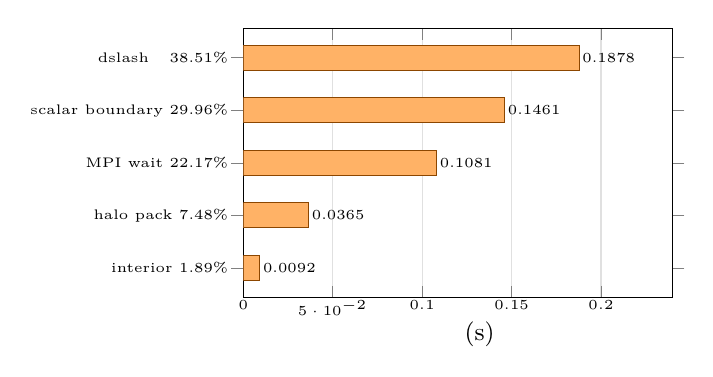
\begin{tikzpicture}
\begin{axis}[
  name=prof,
  width=0.58\linewidth, height=5.0cm,
  xbar, bar width=9pt,
  xmin=0, xmax=0.24,
  xlabel={该阶段耗时 (s)},
  symbolic y coords={interior,halo,wait,boundary,outside},
  ytick=data,
  yticklabels={{interior 1.89\%},{halo pack 7.48\%},{MPI wait 22.17\%},{scalar boundary 29.96\%},{dslash 之外 38.51\%}},
  xmajorgrids, grid style={black!12},
  point meta=explicit symbolic,
  nodes near coords, nodes near coords style={anchor=west},
  enlarge y limits=0.14,
]
\addplot[fill=orange!60,draw=orange!55!black] table[meta=lab] {
  x       y         lab
  0.0092  interior  0.0092
  0.0365  halo      0.0365
  0.1081  wait      0.1081
  0.1461  boundary  0.1461
  0.1878  outside   0.1878
};
\end{axis}
\end{tikzpicture}\hfill
\begin{tikzpicture}
\begin{axis}[
  at={(prof.east)}, anchor=west, xshift=5mm,
  width=0.36\linewidth, height=5.0cm,
  ybar, bar width=17pt,
  ymin=0, ymax=4.4,
  ylabel={占硬件上限比例 (\%)},
  symbolic x coords={hbm155,hbm200,fp155,fp200},
  xtick=data,
  xticklabels={{HBM 1.55\,GHz},{HBM 2.0\,GHz},{FP32 1.55\,GHz},{FP32 2.0\,GHz}},
  xticklabel style={rotate=32,anchor=north east},
  ymajorgrids, grid style={black!12},
  point meta=explicit symbolic,
  nodes near coords, nodes near coords style={inner sep=2pt},
  enlarge x limits=0.16,
]
\addplot[fill=violet!45,draw=violet!55!black] table[meta=lab] {
  x       y     lab
  hbm155  3.35  3.35
  hbm200  2.85  2.85
  fp155   0.52  0.52
  fp200   0.41  0.41
};
\end{axis}
\end{tikzpicture}
\caption{左：y61（32 ranks$\times$12 threads，$24^3\times64$ c64）dslash 剖析分解，dslash 共 84 次调用，四段合计 $0.1461+0.0365+0.1081+0.0092=0.2999$ s（61.49\%），其余 0.1878 s（38.51\%）在 dslash 之外。右：同一运行的 roofline 利用率。建模口径为“每 rank 每次 Schur apply 读一次 source、输出、两个 parity 规范场与 12$\times$12 onsite 矩阵，无 cache 命中折扣”，34 次 apply 折算全局流量 60.51 GiB、算术 86.63 GFLOP，得 149.5 GB/s 与 199.4 GFLOP/s。分母取 384 线程推断上限：HBM 4.458 TB/s（1.55\,GHz）/5.108 TB/s（2.0\,GHz），FP32 SVE 38.09/49.15 TFLOP/s；HBM 两根柱分别是对 1.55 与 2.0\,GHz 上限的比值，FP32 同理。\textbf{结论}：既非带宽受限也非算力受限，主因是 scalar 边界内核与全局同步。}
\end{figure}

\begin{figure}[H]
\centering
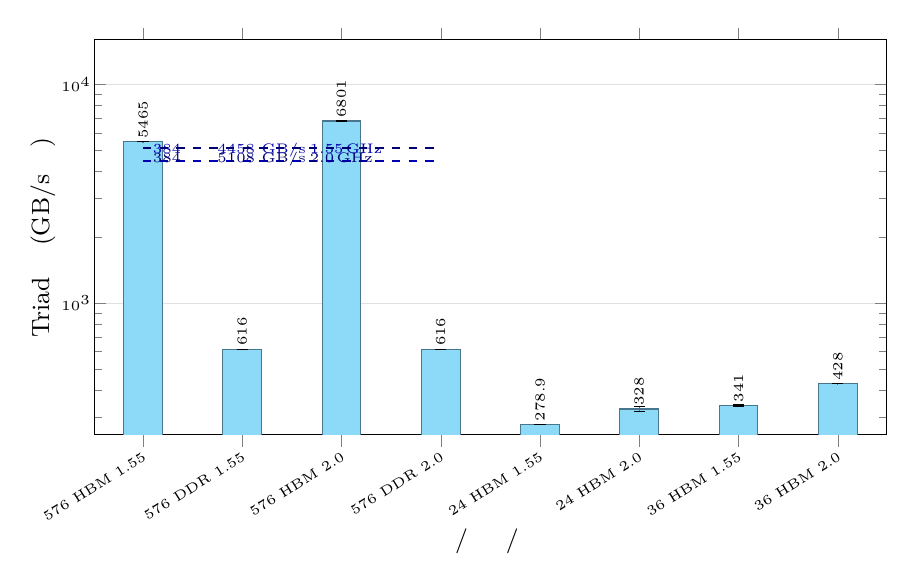
\begin{tikzpicture}
\begin{axis}[
  width=\figw, height=6.6cm,
  ybar, bar width=14pt, ymode=log, log basis y=10,
  ymin=250, ymax=16000,
  ylabel={Triad 带宽 (GB/s，对数轴)},
  xlabel={线程数 / 内存层 / 目标频率},
  symbolic x coords={n576H155,n576D155,n576H200,n576D200,d24H155,d24H200,d36H155,d36H200},
  xtick=data,
  xticklabels={{576 HBM 1.55},{576 DDR 1.55},{576 HBM 2.0},{576 DDR 2.0},{24 HBM 1.55},{24 HBM 2.0},{36 HBM 1.55},{36 HBM 2.0}},
  xticklabel style={rotate=32,anchor=north east},
  ymajorgrids, grid style={black!12},
  point meta=explicit symbolic,
  nodes near coords, nodes near coords style={rotate=90,anchor=west},
  enlarge x limits=0.07,
]
\addplot[fill=cyan!45,draw=cyan!50!black,error bars/.cd,y dir=both,y explicit]
  table[x=x,y=y,y error plus=ep,y error minus=em,meta=lab] {
  x        y        ep     em     lab
  n576H155 5465.49  10.44  10.44  5465
  n576D155 616.11   0.37   0.37   616
  n576H200 6801.06  10.15  10.15  6801
  n576D200 615.83   0.53   0.53   616
  d24H155  278.88   0      0      278.9
  d24H200  328.01   8.95   8.95   328
  d36H155  341.04   2.33   2.33   341
  d36H200  427.67   0.31   0.31   428
};
\draw[dashed,blue!70!black,thick] (axis cs:n576H155,4458.4) -- (axis cs:n576D200,4458.4)
  node[pos=0.02,above,font=\tiny,text=blue!70!black,anchor=south west]{384 线程推断上限 4458 GB/s（1.55\,GHz）};
\draw[dashed,blue!45!black,thick] (axis cs:n576H155,5107.7) -- (axis cs:n576D200,5107.7)
  node[pos=0.02,below,font=\tiny,text=blue!45!black,anchor=north west]{384 线程推断上限 5108 GB/s（2.0\,GHz）};
\end{axis}
\end{tikzpicture}
\caption{LX2 STREAM FP64 Triad 实测（源码与报告：\texttt{refer/kunpeng/lx2-stream-source/}）。口径为自定义 STREAM-style 固定窗口，每配置每操作 5 轮、共同计时窗口 0.15 s，逻辑读写量$\div$窗口时间，\emph{不是}内存控制器实际字节。柱高为样本内最小--最大的中点，误差条为半幅（$n$ 为 5--7 轮）。\textbf{取列更正}：单域 24 线程 1.55\,GHz 的 Triad 是 \textbf{278.88} GB/s（源表该行 Copy 301.33 / Scale 301.44 / Add 278.65 / Triad 278.88）；\texttt{data/kupl\_roofline\_20261106.json} 记的 278.65 与 319.23 分别取自 Add 列，本图按源表更正。全节点 576 线程数据与源表一致。\textbf{限制}：384 线程上限由 16$\times$单域 $t{=}24$ 推算，不是同时运行 384 线程的实测样本；两组频率来自不同样本，差异不能全部归因于频率。}
\end{figure}

\section{HBM 调用：早期失败与后期成功}

\begin{figure}[H]
\centering
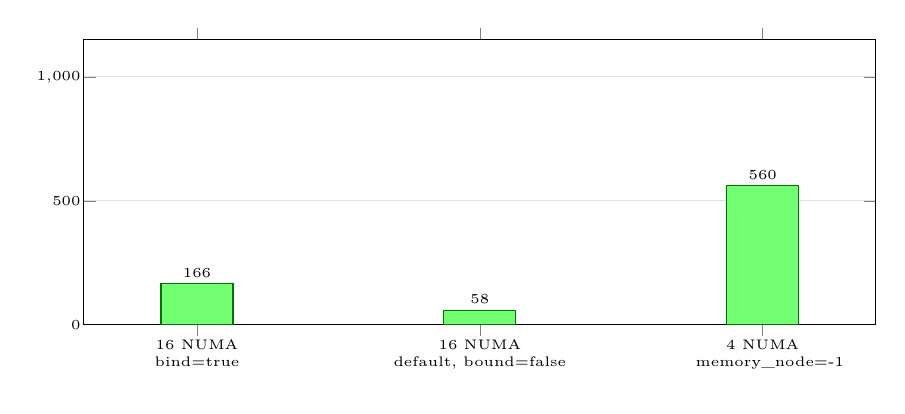
\begin{tikzpicture}
\begin{axis}[
  width=\figw, height=5.2cm,
  ybar, bar width=26pt,
  ymin=0, ymax=1150,
  ylabel={拓扑记录条数},
  symbolic x coords={bindtrue,bindfalse,numanodes4},
  xtick=data,
  xticklabels={{16 NUMA\\bind=true},{16 NUMA\\default, bound=false\\但线程已绑},{4 NUMA\\全部 memory\_node=-1}},
  xticklabel style={align=center},
  ymajorgrids, grid style={black!12},
  point meta=explicit symbolic,
  nodes near coords, nodes near coords style={inner sep=2pt},
  enlarge x limits=0.20,
]
\addplot[fill=green!55,draw=green!45!black] table[meta=lab] {
  x         y    lab
  bindtrue  166  166
  bindfalse 58   58
  numanodes4 560 560
};
\end{axis}
\end{tikzpicture}
\caption{日志中全部 \texttt{PYQCU::KUPL::TOPOLOGY} 记录的统计（共 784 条，\texttt{logs/screen-73056-ss-\dots-*.txt}，等级 A）。\textbf{166 条}为 \texttt{memory\_policy=bind} 且 \texttt{memory\_bound=true}，核心 16 个域到片上内存域 16--31 的配对完整；\textbf{58 条}为 \texttt{memory\_policy=default} 且 \texttt{memory\_bound=false} 但 \texttt{bound\_threads>0}——这类运行只做 CPU 绑定，\emph{不能}计为 HBM 运行；\textbf{560 条}为登录节点的 4 NUMA 记录，\texttt{cpu\_node=-1}、\texttt{cpuset=none}、\texttt{memory\_node=-1}，即根本没有 NUMA/片上内存放置。\textbf{验收边界}：\texttt{memory\_bound=true} 只证明 \texttt{set\_mempolicy()} 调用成功，不等于页实际落在片上内存；严格验收需在 solve 期间用 \texttt{numastat -p} 与 \texttt{/proc/<pid>/numa\_maps} 取证，本项目\textbf{尚未采集}该 live 证据。}
\end{figure}

\begin{figure}[H]
\centering
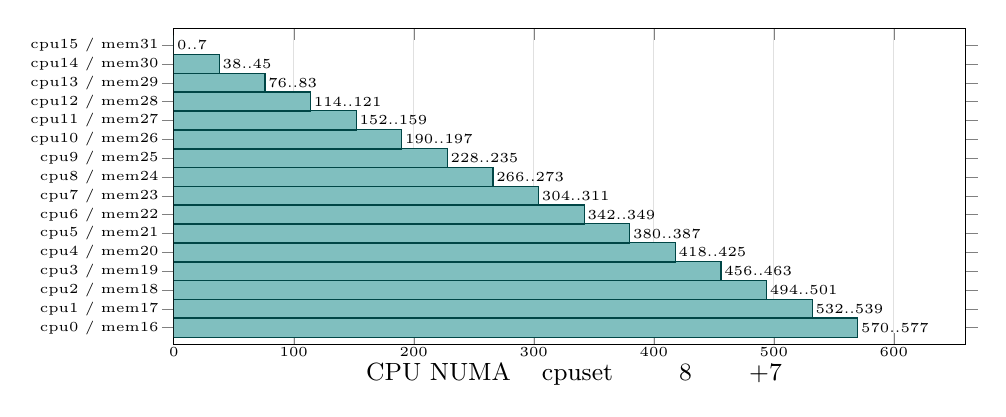
\begin{tikzpicture}
\begin{axis}[
  width=\figw, height=5.6cm,
  xbar, bar width=7pt,
  xmin=0, xmax=660,
  xlabel={该 CPU NUMA 域的 cpuset 起始编号（域内 8 核：起点至起点+7）},
  symbolic y coords={n15,n14,n13,n12,n11,n10,n9,n8,n7,n6,n5,n4,n3,n2,n1,n0},
  ytick=data,
  yticklabels={{cpu15 / mem31},{cpu14 / mem30},{cpu13 / mem29},{cpu12 / mem28},{cpu11 / mem27},{cpu10 / mem26},{cpu9 / mem25},{cpu8 / mem24},{cpu7 / mem23},{cpu6 / mem22},{cpu5 / mem21},{cpu4 / mem20},{cpu3 / mem19},{cpu2 / mem18},{cpu1 / mem17},{cpu0 / mem16}},
  xmajorgrids, grid style={black!12},
  point meta=explicit symbolic,
  nodes near coords, nodes near coords style={anchor=west},
  enlarge y limits=0.06,
]
\addplot[fill=teal!50,draw=teal!55!black] table[meta=lab] {
  x   y    lab
  0   n0   0..7
  38  n1   38..45
  76  n2   76..83
  114 n3   114..121
  152 n4   152..159
  190 n5   190..197
  228 n6   228..235
  266 n7   266..273
  304 n8   304..311
  342 n9   342..349
  380 n10  380..387
  418 n11  418..425
  456 n12  456..463
  494 n13  494..501
  532 n14  532..539
  570 n15  570..577
};
\end{axis}
\end{tikzpicture}
\caption{计算节点 16 个 CPU NUMA 域到片上内存域的实测映射与 cpuset 范围（等级 A，来自 166 条 \texttt{bind=true} 记录）。cpuset 步长恒为 38（每域 38 核，8 线程运行只取前 8 个），最大 CPU 编号 577；$16\times38=608$，与 \texttt{docs/kupl\_kunpeng\_guide.md} 引用的“608 核、每域 38 核”示例机型参数一致。\textbf{注意}：\texttt{memory\_node} 由配置 \texttt{KUPL\_MEMORY\_NODE=local+16} 决定，本图展示“配置生效后的配对”，不是系统自动发现；只在被调度到的运行中出现的域才有记录，故部分域样本数不同（7--22 条）。}
\end{figure}

\section{登录节点筛选（辅助参考，非生产结论）}

\begin{figure}[H]
\centering
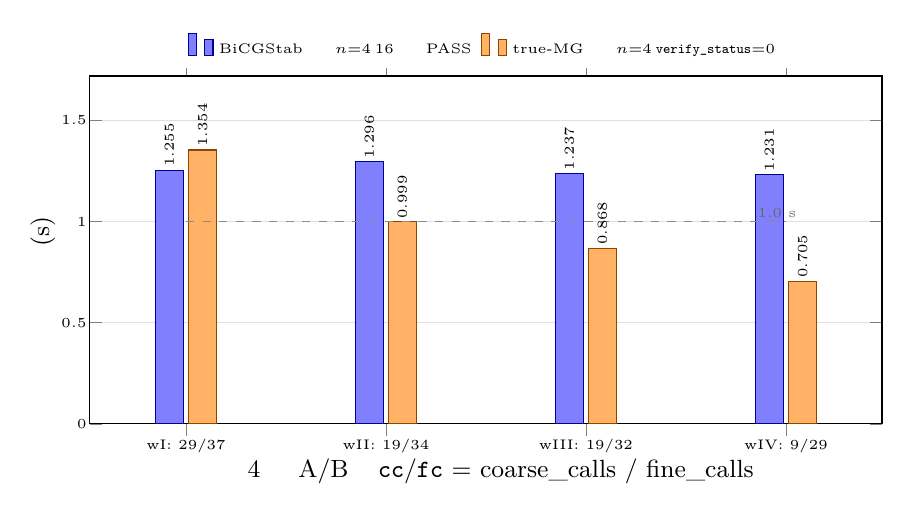
\begin{tikzpicture}
\begin{axis}[
  width=\figw, height=6.0cm,
  ybar, bar width=10pt,
  ymin=0, ymax=1.72,
  ylabel={中位墙钟 (s)},
  xlabel={去重后的 4 个同窗 A/B 窗口（\texttt{cc}/\texttt{fc} = coarse\_calls / fine\_calls）},
  symbolic x coords={wI,wII,wIII,wIV},
  xtick=data,
  xticklabels={{wI: 29/37},{wII: 19/34},{wIII: 19/32},{wIV: 9/29}},
  ymajorgrids, grid style={black!12},
  legend style={at={(0.5,1.02)},anchor=south,legend columns=2,draw=none},
  point meta=explicit symbolic,
  nodes near coords, nodes near coords style={rotate=90,anchor=west},
  enlarge x limits=0.16,
]
\addplot[fill=blue!50,draw=blue!60!black] table[meta=lab] {
  x    y      lab
  wI   1.2546 1.255
  wII  1.2958 1.296
  wIII 1.2370 1.237
  wIV  1.2308 1.231
};
\addlegendentry{BiCGStab 中位（每窗 $n{=}4$，16 迭代，全部 PASS）}
\addplot[fill=orange!60,draw=orange!55!black] table[meta=lab] {
  x    y      lab
  wI   1.3541 1.354
  wII  0.9988 0.999
  wIII 0.8683 0.868
  wIV  0.7051 0.705
};
\addlegendentry{true-MG 中位（每窗 $n{=}4$，\texttt{verify\_status}=0）}
\draw[dashed,black!45] (axis cs:wI,1.0) -- (axis cs:wIV,1.0)
  node[pos=0.97,above,font=\tiny,text=black!60]{持平线 1.0 s};
\end{axis}
\end{tikzpicture}
\caption{登录节点 $24^3\times64$ c64、16 ranks$\times$8 threads、\texttt{grid} $1\,1\,1\,16$、同 gauge/RHS、\texttt{atol}$=10^{-4}$、\texttt{max\_iter}$=50$ 的同窗 A/B（等级 A，本次从屏记录重算）。\textbf{只有 4 个去重窗口}，不是 6 个：\texttt{screen-126} 与 \texttt{screen-127} 的第一窗是同一组 8 个样本，\texttt{screen-128} 与 \texttt{screen-127} 的第二窗也是同一组；\texttt{screen-191/192} 是同一运行的两次偏移 hardcopy，其中 \texttt{bicgstab\_2/3/4}、\texttt{mg\_2/3/4} 六个样本完全相同，只有 \texttt{bicgstab\_1}（1.6147 对 1.3008 s）与 \texttt{mg\_1}（0.6422 对 0.7346 s）不同，因此 wIV 取 191 全集、192 只作复看，未另计窗口。比值 BiCG/MG：wI $0.927$、wII $1.297$、wIII $1.425$、wIV $1.745$（$>1$ 表示 MG 更快）。MAD（BiCG/MG）：wI 0.1018/0.0468；wII 0.0922/0.1818；wIII 0.0472/0.0786；wIV 0.0606/0.0431。\textbf{限制}：全部为共享登录节点，审计时 \texttt{load average}$\approx$91/48、约 106 用户，同配置单样本可在 2.258--1.138 s 间波动；wI 与 wIV 的参数点不同，不得合并为“参数演进收益”。}
\end{figure}

\begin{figure}[H]
\centering
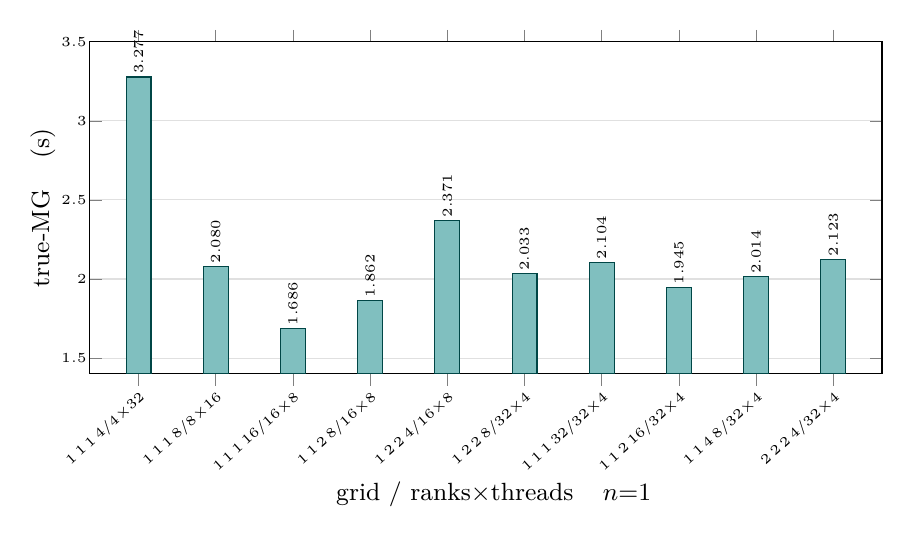
\begin{tikzpicture}
\begin{axis}[
  width=\figw, height=5.8cm,
  ybar, bar width=9pt,
  ymin=1.4, ymax=3.5,
  ylabel={true-MG 墙钟 (s)},
  xlabel={分格 grid / ranks$\times$threads（每点 $n{=}1$）},
  symbolic x coords={g4t,g8t,g16t,g1128,g1224,g1228,g32t,g11216,g1148,g2224},
  xtick=data,
  xticklabels={{$1\,1\,1\,4$/4$\times$32},{$1\,1\,1\,8$/8$\times$16},{$1\,1\,1\,16$/16$\times$8},{$1\,1\,2\,8$/16$\times$8},{$1\,2\,2\,4$/16$\times$8},{$1\,2\,2\,8$/32$\times$4},{$1\,1\,1\,32$/32$\times$4},{$1\,1\,2\,16$/32$\times$4},{$1\,1\,4\,8$/32$\times$4},{$2\,2\,2\,4$/32$\times$4}},
  xticklabel style={rotate=42,anchor=north east},
  ymajorgrids, grid style={black!12},
  point meta=explicit symbolic,
  nodes near coords, nodes near coords style={rotate=90,anchor=west},
  enlarge x limits=0.07,
]
\addplot[fill=teal!50,draw=teal!55!black] table[meta=lab] {
  x       y        lab
  g4t     3.27704  3.277
  g8t     2.07968  2.080
  g16t    1.68634  1.686
  g1128   1.86214  1.862
  g1224   2.37107  2.371
  g1228   2.03263  2.033
  g32t    2.10423  2.104
  g11216  1.94527  1.945
  g1148   2.01389  2.014
  g2224   2.12254  2.123
};
\end{axis}
\end{tikzpicture}
\caption{L24 true-MG 分格扫描（登录节点，每点 $n{=}1$），全部通过 \texttt{KUPL\_REQUIRE\_MG\_CORRECTION} fail-closed 门且 \texttt{verify\_status}$=0$。最优为 $1\,1\,1\,16$ 的 1.68634 s；32 rank 点未进一步加速。\textbf{限制}：单样本；柱间差异同时包含共享负载漂移，只有同窗重复才能定为分格优劣。}
\end{figure}

\begin{figure}[H]
\centering
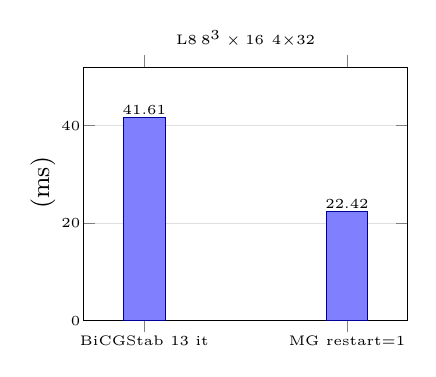
\begin{tikzpicture}
\begin{axis}[
  name=l8,
  width=0.47\linewidth, height=4.8cm,
  ybar, bar width=15pt,
  ymin=0, ymax=52,
  ylabel={墙钟 (ms)},
  symbolic x coords={bicg,mg},
  xtick=data, xticklabels={{BiCGStab 13 it},{MG restart=1}},
  ymajorgrids, grid style={black!12},
  point meta=explicit symbolic,
  nodes near coords, nodes near coords style={},
  enlarge x limits=0.30,
  title={L8（$8^3\times16$），4$\times$32},
]
\addplot[fill=blue!50,draw=blue!60!black] table[meta=lab] {
  x    y     lab
  bicg 41.61 41.61
  mg   22.42 22.42
};
\end{axis}
\end{tikzpicture}\hfill
\begin{tikzpicture}
\begin{axis}[
  at={(l8.east)}, anchor=west, xshift=4mm,
  width=0.49\linewidth, height=4.8cm,
  ybar, bar width=13pt,
  ymin=0, ymax=0.80,
  ylabel={墙钟 (s)},
  symbolic x coords={r4b,r4m,r32b,r32m},
  xtick=data,
  xticklabels={{4$\times$32\\BiCG},{4$\times$32\\MG},{32$\times$4\\BiCG},{32$\times$4\\MG}},
  xticklabel style={align=center},
  ymajorgrids, grid style={black!12},
  point meta=explicit symbolic,
  nodes near coords, nodes near coords style={rotate=90,anchor=west},
  enlarge x limits=0.14,
  title={L16（$16^3\times32$）},
]
\addplot[fill=blue!50,draw=blue!60!black] table[meta=lab] {
  x    y       lab
  r4b  0.70283 0.7028
  r4m  0.16925 0.1693
  r32b 0.16635 0.1664
  r32m 0.16597 0.1660
};
\end{axis}
\end{tikzpicture}
\caption{小格点上 MG 与 BiCGStab 的对比（登录节点，等级 B，源自 \texttt{logs/kupl\_hbm\_opt\_20261106.md} 的 L8/L16 表，\emph{本地无对应 raw JSON}）。L8（$8^3\times16$、4$\times$32）：BiCGStab 0.04161 s（13 迭代）对 MG \texttt{restart=1} 0.02242 s，约 $1.86\times$。L16（$16^3\times32$）：4$\times$32 时 MG 0.16925 s 对 BiCGStab 0.70283 s，约 $4.15\times$；但 32$\times$4 时两者几乎持平（MG 0.16597 s 对 BiCGStab 0.16635 s，约 $1.002\times$），说明粗层工作与小消息同步在 rank 数上升后抵消了迭代优势。\textbf{因此 BiCG 与 MG 必须分格调优}，不能沿用同一 \texttt{grid}。L16 中 16$\times$8 与 32$\times$4 的 MG 分别为 0.13384 / 0.16597 s（同一文档另一表），两张表来自不同分格矩阵，不可逐点混算。}
\end{figure}

\section{Setup 成本、初始化与 opt-in 内核}

\begin{figure}[H]
\centering
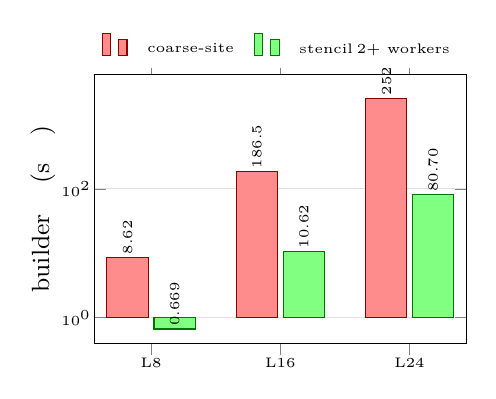
\begin{tikzpicture}
\begin{axis}[
  name=bld,
  width=0.52\linewidth, height=5.0cm,
  ybar, bar width=15pt, ymode=log, log basis y=10,
  ymin=0.4, ymax=6000,
  ylabel={builder 耗时 (s，对数轴)},
  symbolic x coords={L8,L16,L24},
  xtick=data,
  ymajorgrids, grid style={black!12},
  legend style={at={(0.5,1.02)},anchor=south,legend columns=2,draw=none},
  point meta=explicit symbolic,
  nodes near coords, nodes near coords style={rotate=90,anchor=west},
  enlarge x limits=0.22,
]
\addplot[fill=red!45,draw=red!55!black] table[meta=lab] {
  x   y     lab
  L8  8.617 8.62
  L16 186.52 186.5
  L24 2520   2520*
};
\addlegendentry{串行 coarse-site 循环}
\addplot[fill=green!50,draw=green!45!black] table[meta=lab] {
  x   y     lab
  L8  0.669 0.669
  L16 10.62 10.62
  L24 80.70 80.70
};
\addlegendentry{并行 stencil（2+ workers）}
\end{axis}
\end{tikzpicture}\hfill
\begin{tikzpicture}
\begin{axis}[
  at={(bld.east)}, anchor=west, xshift=5mm,
  width=0.43\linewidth, height=5.0cm,
  ybar, bar width=17pt,
  ymin=0, ymax=52,
  ylabel={每 rank 初始化耗时 (s)},
  symbolic x coords={typical,outlier,hbmbind},
  xtick=data,
  xticklabels={{applyInit\\6.02--7.43},{rank 2 离群\\（register 19.48）},{HBM+HugePage\\register 41.75--46.30}},
  xticklabel style={rotate=30,anchor=north east,align=center},
  ymajorgrids, grid style={black!12},
  point meta=explicit symbolic,
  nodes near coords, nodes near coords style={rotate=90,anchor=west},
  enlarge x limits=0.18,
]
\addplot[fill=gray!45,draw=gray!55!black,error bars/.cd,y dir=both,y explicit]
  table[x=x,y=y,y error plus=ep,y error minus=em,meta=lab] {
  x        y      ep    em    lab
  typical  6.725  0.705 0.705 6.73
  outlier  34.81  0     0     34.8
  hbmbind  44.025 2.275 2.275 44.0
};
\end{axis}
\end{tikzpicture}
\caption{左：MG cache builder 串行 vs 并行（\texttt{KUPL\_ENABLE\_MG\_STENCIL\_PARALLEL=1}，默认关闭，等级 B）。加速比 12.9$\times$ / 17.6$\times$ / $>31\times$；L8 与 L16 的 gram/Galerkin 数值完全一致，L24 为 gram $1.55\times10^{-6}$、Galerkin $3.58\times10^{-7}$。\textbf{带星号的 2520 s 是外推值}：由“stencil 1382/27648 用 125.98 s”推得约 42 min，\emph{不是}实测完成值（该次已终止）。右：计算节点初始化（等级 A）。作业 2050850（16 rank，\texttt{END rc=0}，总墙钟 124 s）中 15 个 rank 的 \texttt{applyInit}/\texttt{applyEnd} 为 6.02--7.43 s（柱为中值 6.73 s、半幅 0.71 s），rank 2 为 34.81 s 离群；真实 HBM 运行（y91，\texttt{KUPL\_HUGEPAGE=1}）中 \texttt{register} 升至 41.75--46.30 s（柱为中值 44.03 s、半幅 2.28 s），并出现一次 \texttt{erase} 7.80 s。\textbf{该成本在 \texttt{wall\_seconds} 之外}，必须与求解内核分栏报告。}
\end{figure}

\begin{figure}[H]
\centering
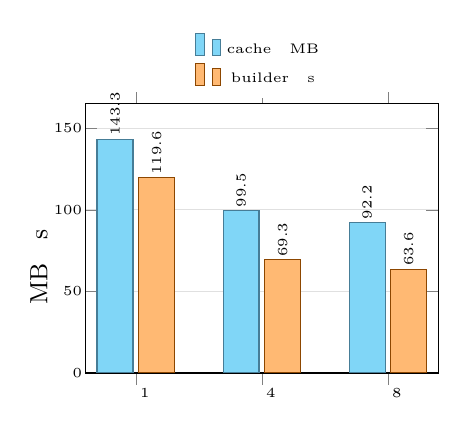
\begin{tikzpicture}
\begin{axis}[
  name=tb,
  width=0.50\linewidth, height=5.0cm,
  ybar, bar width=13pt,
  ymin=0, ymax=165,
  ylabel={指标值（MB 与 s 共用坐标，柱上标单位）},
  symbolic x coords={tb1,tb4,tb8},
  xtick=data, xticklabels={{时间块 1},{时间块 4},{时间块 8}},
  ymajorgrids, grid style={black!12},
  legend style={at={(0.5,1.02)},anchor=south,legend columns=1,draw=none},
  point meta=explicit symbolic,
  nodes near coords, nodes near coords style={rotate=90,anchor=west},
  enlarge x limits=0.20,
]
\addplot[fill=cyan!50,draw=cyan!55!black] table[meta=lab] {
  x   y        lab
  tb1 143.335  143.3 MB
  tb4 99.541   99.5 MB
  tb8 92.242   92.2 MB
};
\addlegendentry{cache 体积（MB）}
\addplot[fill=orange!55,draw=orange!55!black] table[meta=lab] {
  x   y      lab
  tb1 119.57 119.6 s
  tb4 69.33  69.3 s
  tb8 63.59  63.6 s
};
\addlegendentry{builder 耗时（s）}
\end{axis}
\end{tikzpicture}\hfill
\begin{tikzpicture}
\begin{axis}[
  at={(tb.east)}, anchor=west, xshift=5mm,
  width=0.45\linewidth, height=5.0cm,
  ybar, bar width=16pt,
  ymin=0.44, ymax=0.52,
  ylabel={算子内核耗时 (s / 20 次)},
  symbolic x coords={A1,B1,B2,A2},
  xtick=data,
  xticklabels={{A 标量},{B z-lane},{B z-lane},{A 标量}},
  ymajorgrids, grid style={black!12},
  point meta=explicit symbolic,
  nodes near coords, nodes near coords style={},
  enlarge x limits=0.18,
]
\addplot[fill=violet!45,draw=violet!55!black] table[meta=lab] {
  x  y       lab
  A1 0.46023 0.4602
  B1 0.49062 0.4906
  B2 0.49989 0.4999
  A2 0.48491 0.4849
};
\end{axis}
\end{tikzpicture}
\caption{左：L24 时间块对 cache 体积与 builder 成本的影响（等级 B）。时间块 1/4/8 的 cache 分别为 143.3/99.5/92.2 MB（原始字节 143,335,424 / 99,540,992 / 92,241,920），builder 为 119.57/69.33/63.59 s，合法最大 \texttt{grid\_t} 为 32/8/4；三者在 solve 阶段都\emph{慢于}时间块 1，build 节省不抵粗层同步成本。右：\texttt{KUPL\_ENABLE\_T2\_ZBLOCK\_DSLASH=1}（z-lane 向量化）的 A-B-B-A 复测（32 ranks$\times$4 threads，全局 $24^3\times64$，仅 Schur，20 次/块，norm-checked，等级 B）。标量中位 0.47257 s、z-lane 中位 0.49525 s，z-lane 慢 4.8\%；编译器同时报告循环向量化失败，该候选保持 opt-in。}
\end{figure}

\section{证据台账}

\begin{table}[H]
\centering\scriptsize
\caption{本文引用的关键数值及其出处等级。\textbf{A}＝本地可复现原文（屏幕 hardcopy/日志原文）；\textbf{B}＝阶段日志转述（本地无 raw JSON）；\textbf{C}＝文档转述，本地无任何原文。}
\begin{tabularx}{\linewidth}{@{}>{\raggedright\arraybackslash}p{4.3cm}>{\raggedright\arraybackslash}p{3.0cm}>{\raggedright\arraybackslash}X>{\raggedright\arraybackslash}p{0.8cm}@{}}
\toprule
数值 & 含义 & 出处 & 级 \\
\midrule
0.43456275 s / 16 it & y76 计算节点 BiCGStab & \texttt{logs/kupl\_hbm\_opt\_20261106.md}（未入库）；\texttt{logs/v202611061446.txt} & B \\
0.4472 / 0.5719 s & y75 / y74 单样本 & \texttt{logs/resume-20261105T080514.gnF1tz.txt} & B \\
0.4877 / 0.5093 / 0.5126 s & y61 / y50 / y47 & \texttt{logs/kupl\_qcu\_mg\_performance\_reference\_20261105.txt} & B \\
0.475 s & 历史最低（安静节点） & 同上 & B \\
0.9473317482 s & \texttt{restart=50} full-residual & \texttt{logs/screen-73056-ss-20261106-193..195.txt} & A \\
1.23078 / 0.70515 s & 登录节点 r20 窗口中位 & \texttt{screen-\dots-191/192.txt}（本次重算） & A \\
1.2546 / 1.3541 s & 登录节点早期窗口中位 & \texttt{screen-\dots-123.txt}（本次重算） & A \\
1.3972 / 0.78976 s & 文档所记 r10 中位 & \texttt{logs/v20261106104704.txt}；\texttt{screen-127.txt} & A/B \\
1.09187 / 0.70424 s & 文档所记 r50 同窗中位 & 仅 \texttt{logs/v20261106114436.txt} & B \\
213.44090568200045 s & 作业 2050917 的 16$\times$8 求解 & \texttt{screen-1829-bicg-report.txt} & A \\
164.7499241 s & 作业 2049318 的 4$\times$32 求解 & \texttt{logs/kupl\_hbm\_opt\_20261106.md} & B \\
8.617 / 186.52 / 80.70 s & 串行 L8/L16、并行 L24 builder & 同上 & B \\
0.70283 / 0.16925 / 0.16597 s & L16 BiCG/MG@4、MG@32 & 同上 & B \\
89.13 s & 原始基线（4$\times$32，无映射） & 指令日志转述 & C \\
\bottomrule
\end{tabularx}
\end{table}

\begin{table}[H]
\centering\scriptsize
\caption{计算节点作业台账（全部等级 A，调度器记录）。“— ”表示该作业未产生求解报告。}
\begin{tabularx}{\linewidth}{@{}l>{\raggedright\arraybackslash}p{2.0cm}>{\raggedright\arraybackslash}p{1.5cm}>{\raggedright\arraybackslash}p{1.5cm}>{\raggedright\arraybackslash}X>{\raggedright\arraybackslash}p{1.3cm}@{}}
\toprule
作业 & 类型 & ranks$\times$thr & 墙钟 (s) & 结局 & 等级 \\
\midrule
2048748 & 1-rank 探针 & 1$\times$1 & — & 被接受并调度到 cn10579，声明的 \texttt{y79.out} 未生成 & A \\
2048816 & 32-rank A/B & 32$\times$12 & 4894 & host pre-hook 后无 case stdout，同队列 kill，exit 143 & A \\
2048893 & 16-rank 提交 & 16 & — & 被接受但未出现在活动作业查询 & A \\
2049318 & 4-rank A/B & 4$\times$32 & 850 & BiCGStab 164.75 s PASS（native 残差）；配对 MG 10 min 门后 kill，exit 143 & A \\
2049394 & block 路径屏 & 16$\times$8 & 1370 & 仅拓扑输出，exit 143 & A \\
2049477 & slab 路径屏 & 16$\times$8 & 1160 & 仅拓扑输出，exit 143 & A \\
2050223 & t-only 屏 & 32$\times$4 & 540 & 无 report & A \\
2050424 & init 剖析 & 16$\times$8 & 56 & \texttt{END rc=0}，v1 目录 & A \\
2050689 & init 剖析 & 16$\times$8 & 240 & 内部超时 \texttt{rc=124}，停在 topology-report & A \\
2050850 & init 剖析 & 16$\times$8 & 124 & \texttt{END rc=0}，全部 16 rank 完成 & A \\
2050917 & MG 正式 & 16$\times$8 & 787 & 无 \texttt{report.json}，TERM kill-job 2051058，exit 143 & A \\
2051058 & kill-job & 1$\times$1 & — & 同队列本账号 TERM，成功 & A \\
\bottomrule
\end{tabularx}
\end{table}

\end{document}
